\documentclass[numbers=noenddot,12pt,a4paper]{scrartcl}
\usepackage[greek,ngerman]{babel}
\usepackage[T1]{fontenc}
\usepackage[utf8]{inputenc}
\usepackage{fullpage}
\usepackage{libertine}
\usepackage{ziffer}
\usepackage{graphicx}
\usepackage{units}
%\usepackage{wasysym}
\usepackage{amsmath}
\usepackage{amssymb}
\usepackage{wrapfig}
\usepackage{esint}
\usepackage{float}
\usepackage{wrapfig}
\usepackage[font=small]{caption}
\usepackage{subcaption}

\renewcommand{\thefigure}{Abb. \arabic{figure}}

\captionsetup[wrapfigure]{name=}
\captionsetup[figure]{name=}
\newcommand{\degree}{^\circ}
\newcommand{\diff}{\textnormal{d}}
\newcommand{\tenpo}[1]{\cdot 10^{#1}}
\newcommand{\greek}[1]{\greektext#1\latintext}
\newcommand{\ix}[1]{_\text{#1}}
\newcommand{\imag}{\mathbf{i}}

\title{Protokoll: Digitale Schaltungen}
\author{Tom Kranz, Philipp Hacker}
\date{\today}

\begin{document}
%\setcounter{page}{2}
%\setcounter{section}{1}
\maketitle
\vspace*{\fill}
\tableofcontents
\vfill
\newpage
\section{Schaltskizzen}
\begin{figure}[H]
\centering
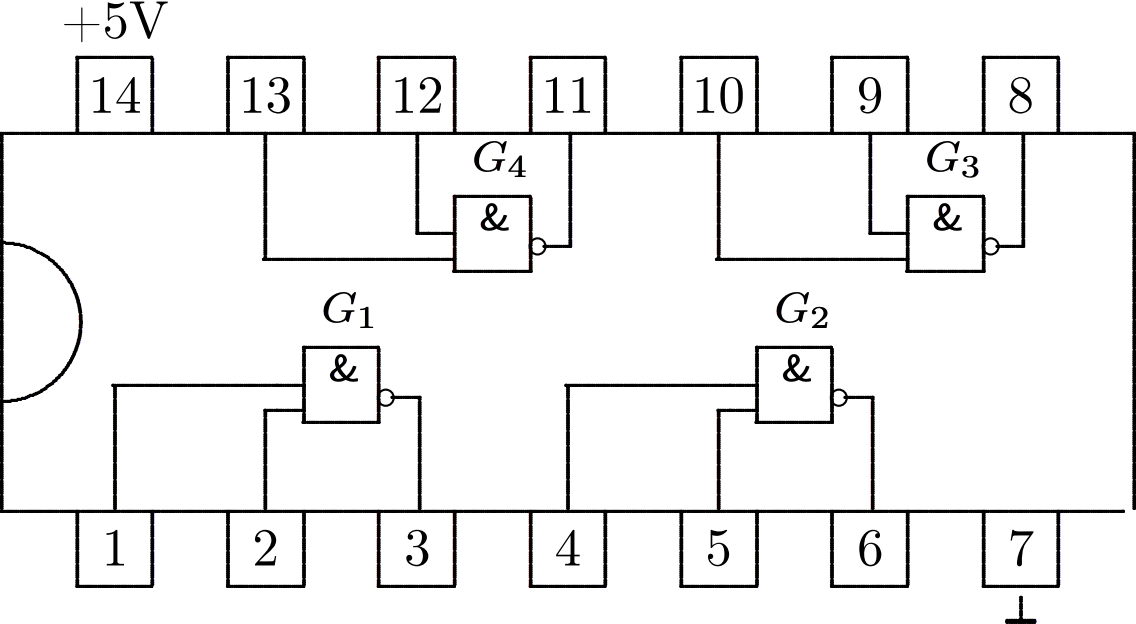
\includegraphics[width=0.666\textwidth]{NANDIC.png}
\caption{IC SN 7400 bzw. SN 74HCT00} \label{img:ic}
\end{figure}
\section{Durchführung}
\subsection{Versuchsaufgabe 1}
Hierbei wurden die beide Eingänge eines NAND-Gatters mit einem Signal $U\ix{x}$ beschaltet. Zuerst wurde der Verlauf des Ausgangssignals $U\ix{y}$ bei den quasistatischen Variationen $U\ix{x}=0\rightarrow\unit[5]{V}$ und $U\ix{x}=5\rightarrow\unit[0]{V}$ mittels Multimetern gemessen Anschließend wurde für das Eingangssignal ein systemeigener Rechteckimpuls der Frequenz $1$ bzw. $\unit[10]{MHz}$ eingesetzt. Systemeigen bedeutet hierbei, dass ein Gatter zwischen ursprünglicher Spannungsquelle und Eingang des Messgatters geschaltet war. Der Rechteckimpuls hatte eine Peak-to-Peak-Spannung von $\unit[5]{V}$ mit einem Offset von $\unit[2,5]{V}$. Ein- und Ausgangssignal wurden zeitsynchron oszillographiert.
\subsection{Versuchsaufgabe 2}
Für 2 unterschiedliche ICs (siehe \ref{sec:gerät}) wurde die Verlustleistung in Abhängigkeit von der Frequenz des ansteuernden systemeigenen Rechteckimpulses gemessen. Dabei wurde die Stromaufnahme mit freien Gattern, d.h. alle Gatter sind ohne Ein- bzw. Ausgangssignal, und mit beschalteten Gattern gemessen.
\subsection{Versuchsaufgabe 3}
Wie in \ref{img:ic} gezeigt, können beliebig Ein- bzw. Ausgänge von Gattern in einem IC miteinander verschaltet werden. Hierbei sollte nun, nacheinander für die ICs aus \ref{sec:gerät}, bis zu 3 Gatter in Reihe geschaltet werden. Gemessen wurde die Ausgangsspannung des 1. Gatters, welches für jede Schaltung mit einem High $U\ix{H}$ und einem Low $U\ix{l}$ auf beiden Eingängen angesteuert wurde. \\
Für die Schaltung mit keinem nachgeschalteten Gatter wurden die Eingänge \textbf{1} und \textbf{2} zusammengelegt und, wie in allen anderen Schaltungen auch, der Ausgang \textbf{3} gemessen. Mit einem Gattern wurde der Ausgang \textbf{3} zusätzlich auf die Eingänge \textbf{4} und \textbf{5} gelegt. Für 2 Gatter wurde das Signal aus \textbf{3} wiederum auf \textbf{9} bzw. \textbf{10} geschaltet. Schließlich wurde für 3 Gatter das Ausgangssignal aus \textbf{3} auf alle Eingänge des ICs weitergegeben (für Nummerierung siehe \ref{img:ic}).
\subsection{Geräte} \label{sec:gerät}
Die verwendete Versuchsplatine ist "`Logisches Gatter"'. Die Betriebsspannung und die verschiedenen Eingangs-Gleichspannungen lieferte das Stromversorgungsgerät \textsc{Tektronix PS 280}, Rechtecksignale wurden mit dem Funktionsgenerator \textsc{Tektronix AFG 3022B} erzeugt. Die Gleichspannungen wurden mit dem Multimeter \textsc{VOLTCRAFTplus VC 920} gemessen, Oszillogramme und Signalverläufe mit dem Oszilloskop \textsc{Hameg HM1508-2} erstellt bzw. betrachtet.
\subsection{Oszillogramme}
\subsubsection{Versuchsaufgabe 1}
\begin{figure}[H]
\centering
\begin{subfigure}[b]{0.48\textwidth}
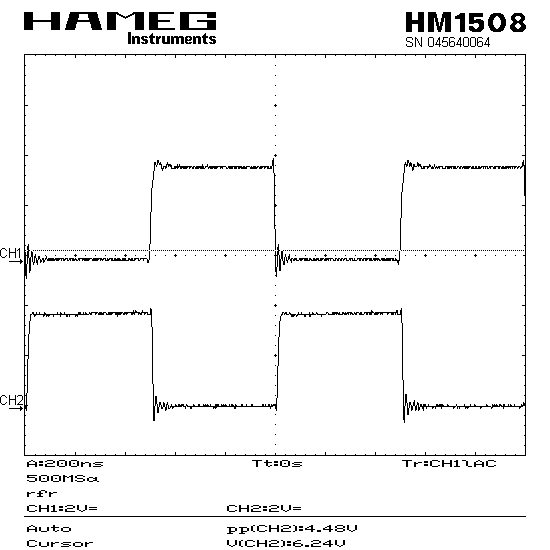
\includegraphics[width=\textwidth]{scr16.png}
\caption{$f=\unit[1]{MHz}$} \label{img:osz1}
\end{subfigure}
\begin{subfigure}[b]{0.48\textwidth}
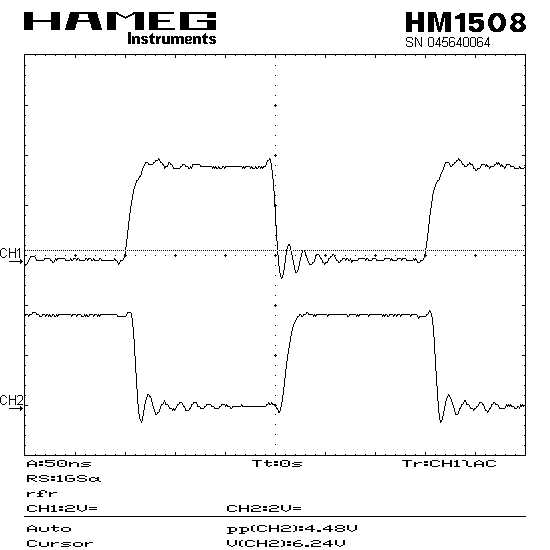
\includegraphics[width=\textwidth]{scr17.png}
\caption{$f=\unit[10]{MHz}$} \label{img:osz2}
\end{subfigure}
\caption{zeitsynchrone Ein- und Ausgangssignale (systemeigen, Rechteckimpuls)}
\end{figure}
\section{Auswertung}
\subsection{Versuchsaufgabe 1}
\begin{figure}[H]
\centering
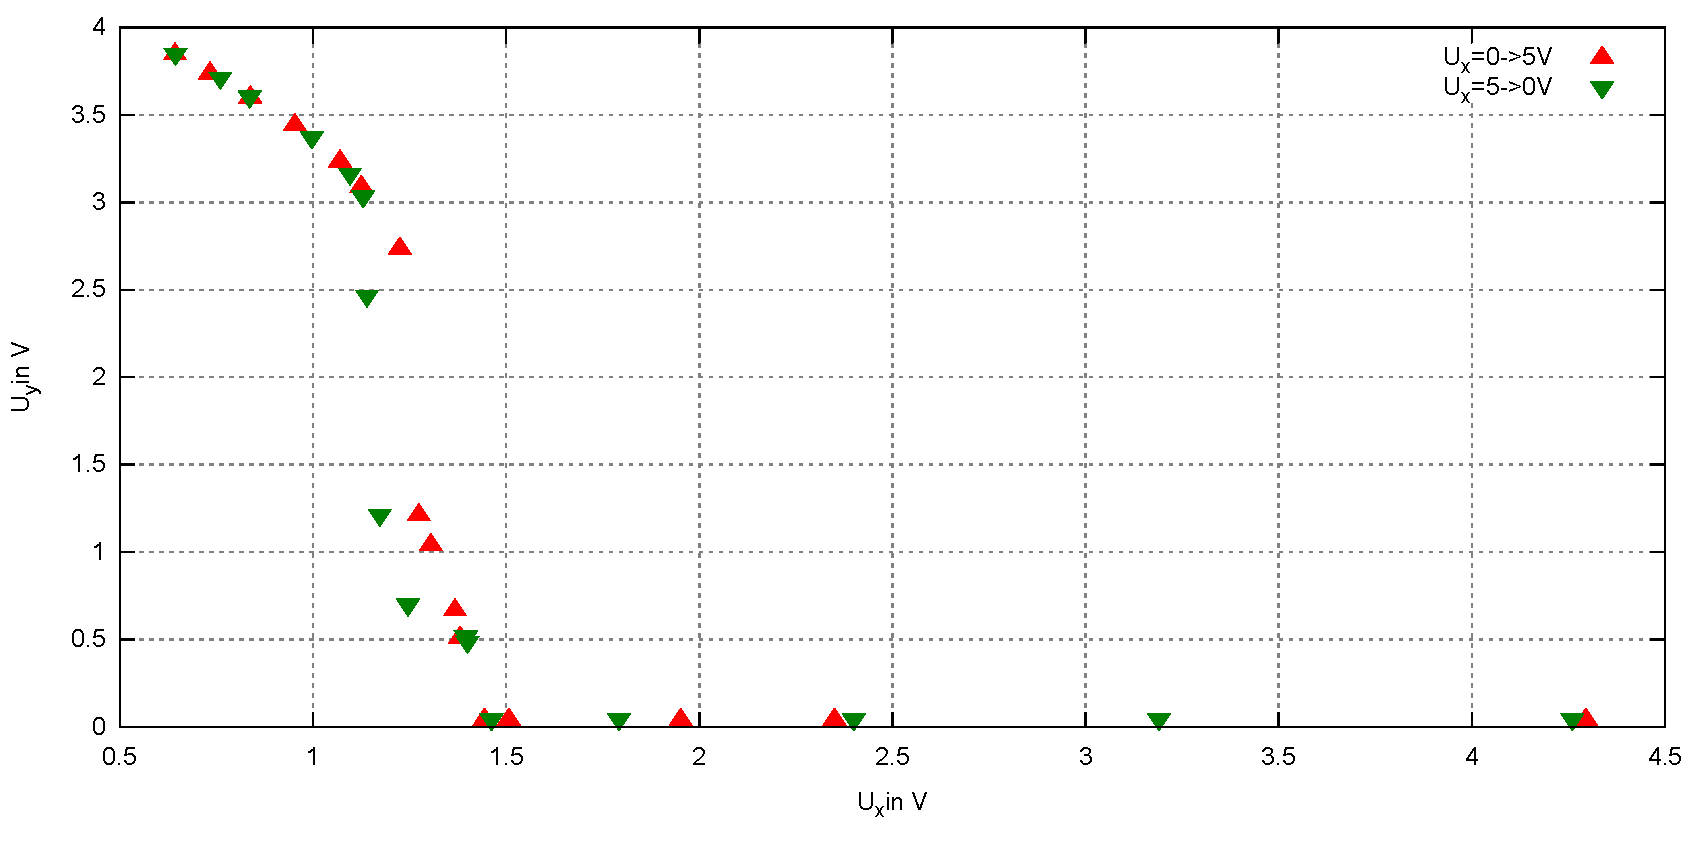
\includegraphics[width=0.666\textwidth]{aufg1.pdf}
\caption{Ausgangssignal eines Gatters bei variierendem Eingangssignal}
\end{figure}
Im gezeigten Diagramm ist der Umbruch von High- zu Low-Pegel zu erahnen. Die verbotene Zone sollte jedoch keine Messwerte liefern (\unit[0,4\dots 2,4]{V}). \\
Aus den Oszillogrammen \ref{img:osz1} und \ref{img:osz2} ergibt sich die Laufzeit zu
\begin{align*}
\tau=\frac{\tau\ix{HL}+\tau\ix{LH}}{2}=\frac{\unit[\left(1,47036-1,3963\right)]{10^{-7}s}+\unit[\left(100,29-4,634\right)]{10^{-10}s}}{2}=\unit[8,4858]{ns} \; .
\end{align*}
\subsection{Versuchsaufgabe 2}
Da für ein einziges Gatter die Verlustleistung nicht messbar war, betrachten wir die über den gesamten IC abfallenden Leistung. Dafür wurde der eingehende Strom und die Speisespannung in Abhängigkeit vom Eingangssignaltakt gemessen. Während der Messung waren alle 4 Gatter frei, d.h. nicht beschaltet. Die gesuchte Leistung ist $P\ix{V}=\frac{P\ix{ges}}{4}$.
\begin{table}[H]
\centering
\begin{tabular}{c||c|c|c|c}
 IC & $U\ix{s}\unit{/V}$ & $I\ix{s}\unit{/mA}$ & $f\unit{/kHz}$ & $P\ix{V}\unit{/mW}$ \\ \hline \hline 
SN7400 & 4,98 & 30,989 & 0 & 0,198\\ \cline{3-5}
 &  & 31,02 & 1 & 0,1544 \\ \cline{3-5}
 &  & 31,42 & 10000 & 0,1564 \\ \cline{1-5}
SN74HCT00 & 4,98 & 36,38 & 0 & 0,1811 \\ \cline{3-5}
 &  & 32,54 & 1 & 0,1621 \\ \cline{3-5}
 &  & 35,334 & 10000 & 0,1759
\end{tabular} 
\end{table}
\subsection{Versuchsaufgabe 3}
\begin{figure}[H]
\centering
\begin{subfigure}[b]{0.48\textwidth}
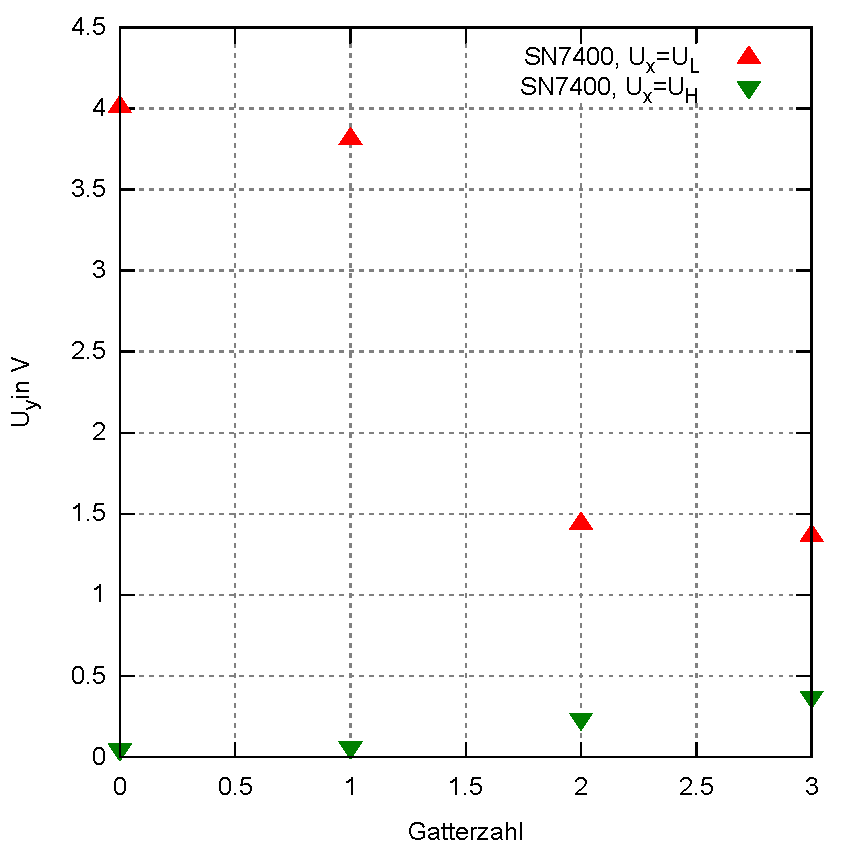
\includegraphics[width=\textwidth]{aufg3_1.pdf}
\end{subfigure}
\begin{subfigure}[b]{0.48\textwidth}
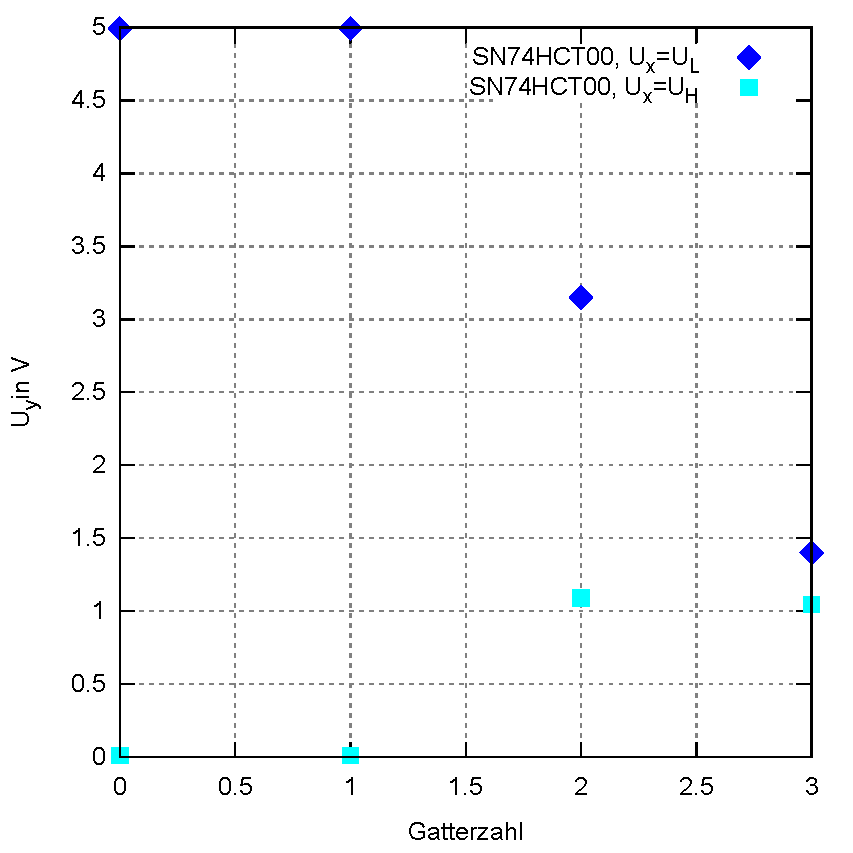
\includegraphics[width=\textwidth]{aufg3_2.pdf}
\end{subfigure}
\caption{Ausgangsspannung bei steigender Belastung (Vergleich der ICs)}
\end{figure}
Der Ausgangslastfaktor eines Gatters (fan-out) gibt an, wie viele, in ihrem Eingangslastfaktor (fan-in) gleichwertige, Gatter angeschlossen werden können, ohne dass das Ausgangssignal den High- bzw. Low-Bereich verlässt. In unserem Fall handelte es sich um ein NAND-Gatter - d.h. dass aus einem, auf beiden Eingängen anliegenden, High am Ausgang ein Low wird und umgekehrt. Der Low-Pegel ist $U\ix{L}\in \left[0\dots  \unit[0,4]{V}\right]$ und der High-Pegel $U\ix{H}\in \left[2,4\dots \unit[5]{V}\right]$. \\
Für das Gatter des ICs SN7400 wird damit ersichtlich, dass dessen fan-out zwischen 1 und 3 liegen muss. Das Gatter aus dem SN74HCT00 besitzt den Messergebnissen zur Folge einen ähnlichen fan-out. Diese Ergebnisse stehen aber im Widerspruch zu den Annahmen, dass ein fan-out dieser TTL-Gatter etwa 10 betragen sollte. 
\section{Anhang}
Die originalen Messwert-Aufzeichnungen liegen bei.
\end{document}